% TEMPLATE for Usenix papers, specifically to meet requirements of
%  USENIX '05
% originally a template for producing IEEE-format articles using LaTeX.
%   written by Matthew Ward, CS Department, Worcester Polytechnic Institute.
% adapted by David Beazley for his excellent SWIG paper in Proceedings,
%   Tcl 96
% turned into a smartass generic template by De Clarke, with thanks to
%   both the above pioneers
% use at your own risk.  Complaints to /dev/null.
% make it two column with no page numbering, default is 10 point

% Munged by Fred Douglis <douglis@research.att.com> 10/97 to separate
% the .sty file from the LaTeX source template, so that people can
% more easily include the .sty file into an existing document.  Also
% changed to more closely follow the style guidelines as represented
% by the Word sample file. 

% Note that since 2010, USENIX does not require endnotes. If you want
% foot of page notes, don't include the endnotes package in the 
% usepackage command, below.

% This version uses the latex2e styles, not the very ancient 2.09 stuff.
\documentclass[letterpaper,twocolumn,10pt]{article}
\usepackage{epsfig,graphicx,usenix,fullpage, hyperref}


%\usepackage{endnotes}
\begin{document}

%don't want date printed

%make title bold and 14 pt font (Latex default is non-bold, 16 pt)
\title{\Large \bf 6.829 Final Project: A comparison of bit-rate selection algorithms}
%for single author (just remove % characters)
\author{
{\rm Colleen Josephson}\\
cjoseph@mit.edu
\and
{\rm Pavel Panchekha}\\
pavpan@mit.edu
% copy the following lines to add more authors
% \and
% {\rm Name}\\
%Name Institution
} % end author

\date{May 2013}

\maketitle

% Use the following at camera-ready time to suppress page numbers.
% Comment it out when you first submit the paper for review.
%\thispagestyle{empty}

\subsection*{Abstract}
In this paper we compare the performance SampleRate and Minstrel, two popular bit rate selection algorithms that have widespread real-world usage on the Linux operating system. We use a novel trace-based approach that allows us avoid in-depth kernel programming and write simple Python scripts instead. We also introduce improvements to the Minstrel algorithm that allow for significant gains in throughput. 
\section{Introduction}

One of the key ways that wireless networks differ from wired is that wireless networks have varying link rates. Link conditions vary with time due to interference from other devices, changing network geometry, and mobile clients. An optimal rate at some time $t$ may be different from the optimal rate just 30 seconds earlier. A good bit rate selection algorithm has to detect and adapt to these conditions. If the chosen bit rate is too slow, then the throughput will be unnecessarily low. If the rate is too high, then failures will be very frequent and throughput will again suffer. 

There are three main classes of bit rate adaptiation protocols: frame-based, SNR-based, and cross-layer protocols. Frame-based protocols measure the fraction of sucessfully received protocols. SNR protocols make decisions based on the estimated Signal to Noise ratio. Cross-layer protocols use SoftPHY data from the physical layer. The most commonly implemented protocols on today's networks are frame based, because SNR protocols perform poorly~\cite{samplerate}, and cross-layer protocols cannot be deployed on current networks because they violate the network layering abstration. 

The two most popular fram-based protocols are SampleRate and Minstrel. Both were implemented in the MadWifi drivers for Linux wirless, and today Minstrel is the default bit-rate selection algorithm for all wireless drivers on Linux. Our research used a trace-based approach to analyze the performance of these two algorithms. We also created a modified version of Minstrel that provides significant throughput gains over the vanilla Minstrel implementation. 

This paper will provide a general overview of SampleRate and Minstrel. We then discuss our testing methodology. We compare the performance of the two algorithms, and then discuss modifications we made to Minstrel and compare it's performance to the current kernel implementation.
\section{SampleRate}

SampleRate has three main functions: \texttt{ApplyRate()}, which returns a the bit-rate to send a packet at, \texttt{ProcessFeedback()}, which updates the statistics for a bitrate after an attempted packet send,  and \texttt{RemoveStaleResults()}, which removes all statistics older than 10 seconds.

SampleRate sends at the rate with the lowest average transmission time. Every ten packets, it sends out a sample packet at a random rate that has a smaller predicted transmission time than the current rate. SampleRate updates its transmission time estimates every ten seconds based on feedback from the card about which packets succeeded and at which rate they were sent. If the current best rate experiences four successive failures, SampleRate stops using that rate. 

\section{Minstrel}

Minstrel utilizes the multi-rate retry chain (mrr), which is an array that tells the card which rates to try before reporting a failure. The retry chain makes failures extremely unlikely. Minstrel has a mrr of [\emph{highest throughput, next highest throughput, best probability, lowest base rate}] for most packets. In essence, Minstrel tells the card to send at the highest throughput rates but to fall back to reliable rates upon failure. The throughput and success probability are calculated for each rate every 100ms. 
To keep an accurate estimate of throughput and probability for each rate, Minstrel sends sample frames ten percent of the time. If the randomly chosen rate has a higher lossless throughput than the current optimal rate, the mrr is as follows: [\emph{random, highest throughput, best probability, lowest base rate}]. If the random rate is slower than the optimal rate, it is moved further back in the retry chain: [\emph{best throughput, random, best probability, lowest base rate}]. This ensures that Minstrel never samples rates worse than the current optimal rate unless the optimal rate experiences a failure. See table ~\ref{table:1} for an overview of the mrr's used in Minsterl.

Minstrel's implementation is based on SampleRate's, so it also has \texttt{ApplyRate()} and \texttt{ProcessFeedback()}, as well as a \texttt{UpdateStats()} method that runs every 100ms. \texttt{UpdateStats()} is home to some of the key differences between Minstrel and SampleRate. Instead of making decisions based on the average 
transmission time, Minstrel uses throughput: \begin{equation} T = \frac{p}{tx\_time}\end{equation} where $T$ is the throughput of some rate $r$, $p$ is the probability of successfully transmitting at $r$, and $tx\_time$ is the lossless transmission time at $r$.

The probability $p$ of a successful transmission is calculated from statistics collected by the \texttt{ProcessFeedback()} method, and is done using an exponential weighted moving average, or EWMA. The EWMA creates a weighted average that weighs recent data more heavily than old data. The weighting for old data decreases exponentially. An EWMA is beneficial because it ensures that a sudden degredation in link quality will create a rapid response in the probabilities due to the increased weight of recent data. Minstrel will waste less time sending packets at a rate that no longer works, as compared to a simple probability calculation.

\begin{table*}[htb]
  \centering
    \begin{tabular}[htb]{l|l|l|l}
    \textbf{Try} & \textbf{Normal}               & \textbf{Random (slower than best)} & \textbf{Random (faster than best)} \\ \hline
    1   & Best throughput      & Best throughput           & Random                    \\
    2   & Next best throughput & Random                    & Best throughput           \\
    3   & Highest probability  & Highest probability       & Highest probability       \\
    4   & Lowest rate          & Lowest rate               & Lowest rate               \\
    \end{tabular}
    \caption{Multi-rate retry chains for Minstrel}
\label{table:1}
\end{table*}

\section{Methodology}

We used a trace-based approach to collect data, and then replayed that data to the rate-selection algorithms using a Python framework.

\subsection{Motivation}

Our initial plan was to use the algorithms as implemented in the MadWifi drivers for the Atheros chipset. However, MadWifi is depricated, and only runs on quite old network cards. In addition to the lack of compatible hardware available to us, MadWifi is not an accurate reflection of what a modern user would use. We looked into the ath5k and ath9k projects, which were created to replace MadWifi. Both of these did not port the old bit-rate selection system from MadWifi and instead opted to use the linux kernel's rate selection software, which only offers Minstrel. Porting SampleRate over to the new drivers would not have been trivial, as there are vast differences in the assumed interfaces. 

At this point, we decided to take a different approach and use an approach similar to that used in Sprout~\cite{sprout}.


\subsection{Trace Collection}

TODO

\begin{figure}[hbt]
  \hspace{-0.5em}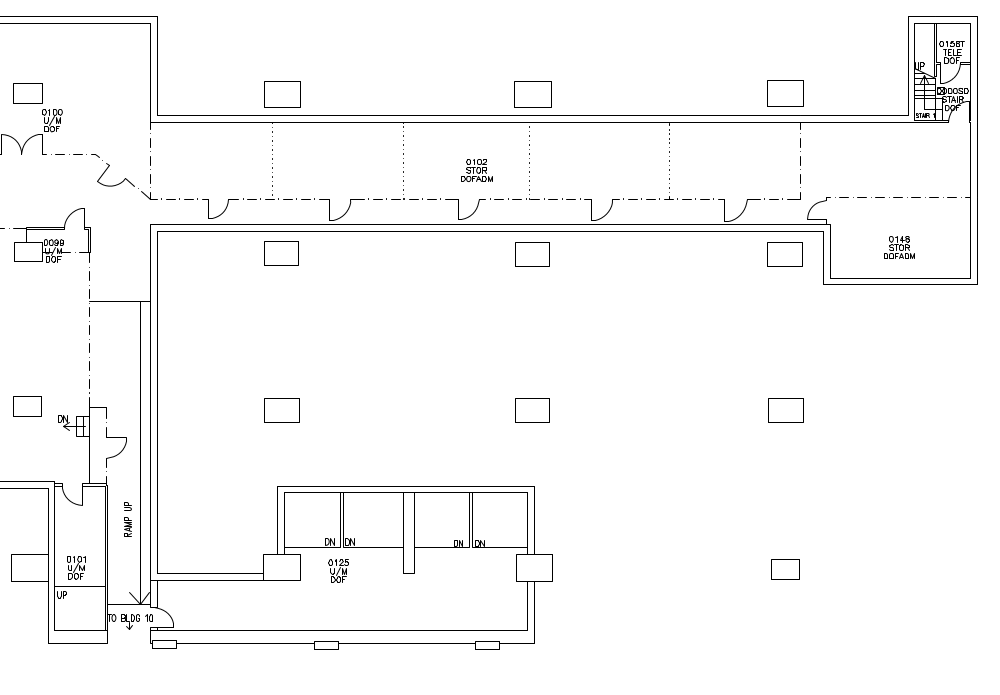
\includegraphics[width=3.5in]{bsmt13floorplan.png}\vspace{-0em}
  \caption{We collected most traces at a remote access point in the basement of Building 13 at MIT.}
\label{figure:1}
\end{figure}

\subsection{Testing framework}

TODO: Harness.py, etc.

We implemented SampleRate as outlined in John Bicket's Master's thesis~\cite{samplerate}. This implementation is slightly different from how it was implemented in the MadWifi kernel driver. The primary difference is that the kernel implementatiion uses a EWMA instead of a 10 second window. The thesis implmenentation throws out old rate data and begins anew every 10 seconds. It would be worth looking at the performance of EWMA-based SampleRate in the future. 

\texttt{samplerate.py} contains \texttt{ApplyRate()}, \texttt{ProcessFeedback()} and  \texttt{RemoveStaleResults()}, as well as a few helper functions and data structures for tracking rate statistics. 

We implemented Minstrel by porting the C code from the 3.3.8 version of the Linux kernel into Python. \texttt{minstrel.py} contains \texttt{ApplyRate()}, \texttt{ProcessFeedback()} and  \texttt{UpdateStats()}, as well as a few helper functions and data structures for tracking rate statistics. 


\section{Analysis}

Minstrel and SampleRate perform similarly, usually within 3 Mbps of each other. In especially noisy situations, such as when the client is moving or when the client is around the corner from the access point, Minstrel consistently outperforms SampleRate. Figure~\ref{figure:3} shows the results of a single run of both Minstrel and SampleRate over all the different types of traces we collected. This is consisten with the literature--the authors of Minstrel noted that they focused on making Minstrel robust to poor conditions~\cite{minstrel}, which means losing potential througput gains in stable situations. Conversely, John Bicket noted that SampleRate performs better in stable situations than noisy or highly varying conditions~\cite{samplerate}. We were slightly surprised to see how significantly SampleRate outperformed Minstrel in certain situations, though, with throughput being up to 67\% higher. 

In Figure~\ref{figure:2} we show the performance of constant bitrates on the \texttt{clear\_1.dat} trace, which is a 35 second trace in clear view of the access point. The optimal rate here was 18 Mbps, which achieved an average throughput of about 15 Mbps. The next highest bitrate, 24 Mbps, shows a large plummet in performance, down to a throughput of 1.17 Mbps. This steep drop is charateristic, and is also talked about in the SampleRate thesis~\cite{samplerate}. It demonstrates just how important bit rate selection is--the optimal bit rate has typically much higher throughput than the next-best rate, but if the algorithm strays too high the results can be devistating. 

Bit rate selection algorithms strive to have a throughput near or greater than the optimal constant rate. For this \texttt{clear\_1.dat} trace, SampleRate clearly meets this goal, achieving an average throughput more than 1 Mbps higher than the optimal constant rate. In noisier situations, though, Minstrel tends to be closer to the optimal constant rate. 

We did notice that Minstrel occasionally has very poor performance on traces 1 seconds or shorter--sometimes as low as 2mbps. This is because it does not stop sending after four successive failures, but must wait until the end of the 100ms window for statistics to be compiled. Thus it wastes a lot of time sending at non-optimal rates, and a short trace only has a few windows. This behavior does not show up in long traces at all, however, as Minstrel has had time to both smooth out bad windows and collect more statistics (making it less likely to choose a bad rate).


Bit rate selection algorithms naturally show variation between runs on the same data because probe rates are chosen randomly. The variations were small, though. On ten runs on the \texttt{clear\_1.dat} trace, the average of Minstrel over 10 runs was 7.52 Mbps, with a maximum variation of +/- 0.12 Mbps. SampleRate was similarly stable, it averaged 5.284 Mbps over 10 runs, with a maximum variation of about +/- 0.3 Mbps. The variation of results on other traces was similar.

The histograms of which rates the algorithms deided to send at provided some useful insight into the behavior. Table~\ref{table:2} is a histogram of a 35 second corner trace. In this situation Minstrel outperforms SampleRate. The constant rate throughputs demonstrate that 11, 12 and 18 Mbps were the optimal rates to send at, and that no packets were sucessful at any higher rates. SampleRate does not use these rates except for probe packets, which happens once every ten seconds. Minstrel does not have this measure, however, spends a lot of time sending probe packets at these high rates that happen to never be successful. The only reason low rates have fewer probe packets is because they are second in the retry chain. Despite the fact that SampleRate spends less time probing high rates, it is less successful. This is because Minstrel send the most packets at the three most successful bitrates. SampleRate, however, spends too much time sampling low bit rates. Additionally, it spends a lot of time sending at 5.5 Mbps. TODO: why does SampleRate spend time at 5.5 Mbps??? We suspect that this might be because the equation SampleRate uses to estimate average transmission time needs to be tweaked. 

Our examination of the histograms showed us that Minstrel spends a lot of time sampling at high rates. In the specific case we examined, they were all probe packets. But sometimes Minstrel would choose 54Mbps as the rate with the best throughput, which made little sense. A closer investigation revealed that Minstrel would sometimes luck out and get one success sending a probe at 54Mbps. The probability of success would be 1, so then 54Mbps would be chosen as the rate with the best throughput. This is unfortunate, but the real harm came in the next window: nearly all of the packets at 54Mbps would fail, but Minstrel was still considering 54 Mbps to be the best rate! This is because the EWMA did not account for the fact that the second block having sent hunreds more packets at 54 Mbps than the first. Thus the probability of success would drop from 1 to about 0.70, which is still high enough for the throughput equation to rank 54 Mbps highly. In essense, the probabilities were not declining fast enough after a large number of failures.

In the next section we will talk about Minproved, an improved version of Minstrel where we attempt to fix the probability problem. 

\begin{figure}[htb]
  \hspace{-1em}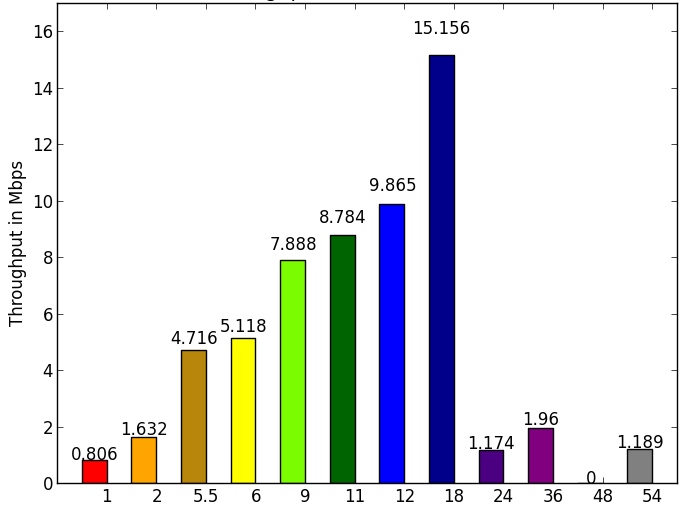
\includegraphics[width=3.4in]{constant.png}\vspace{-0em}
  \caption{Throughput of using a constant 802.11b/g bitrate in clear line-of-sight from the access point.}
\label{figure:2}
\end{figure}


\begin{figure}[htb]
  \hspace{-.75em}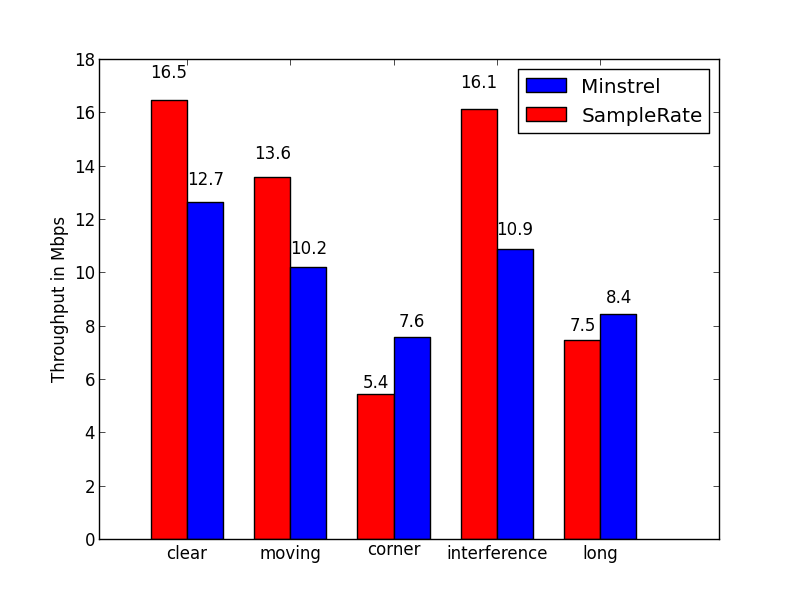
\includegraphics[width=3.5in]{MinVSSam1.png}\vspace{-0.75em}
  \caption{Throughput of Minstrel and SampleRate on various trace situations.}
\label{figure:3}
\end{figure}


\subsection{Improvements to Minstrel}
TODO: Minproved.
-make sure we mention how Minproved almost always does better than highest fixed rate
\begin{table*}[htb]
    \centering
    \begin{tabular}{l|l|l|l|l}
    \textbf{Rate in Mbps}     & \textbf{SampleRate} & \textbf{Minstrel}   & \textbf{Minproved}   & \textbf{Constant Rate Throughput}\\ \hline
    1                & 631        & 39         & 29      & 0.639 Mbps    \\
    2                & 863        & 82         & 20      & 1.425 Mbps    \\
    5.5              & 4814       & 110        & 805     & 4.406 Mbps    \\
    6                & 423       & 137        & 276     & 4.603 Mbps    \\
    9                & 553         & 327        & 57      & 4.630 Mbps   \\
    11               & 3326       & 4121       & 3356    & 9.627 Mbps   \\
    12               & 4649       & 9515       & 14285   & 9.444 Mbps   \\
    18               & 1154         & 13295      & 15795   & 8.458 Mbps    \\
    24               & 16         & 6909       & 1918    & 0 Mbps   \\
    36               & 16         & 6944       & 2030    & 0 Mbps   \\
    48               & 16         & 6888       & 2009    & 0 Mbps   \\
    54               & 16         & 7308       & 1953    & 0 Mbps   \\ \hline
    \textbf{Avg. Throughput:} & \emph{5.42 Mbps}  & \emph{7.578 Mbps} & \emph{11.107 Mbps} \\
    \end{tabular}
    \caption{Histograms of the number of packets sent at each rate.  The trace was \texttt{corner\_1.dat} and was recorded around the corner from the access point. The best fixed rate for this trace was 11 Mbps, which achieved a throughput of 9.627 Mbps. Minproved achieves a higher throughput than the best fixed rate.}
\label{table:2}
\end{table*}

\begin{figure}[htb]
  \hspace{-2em}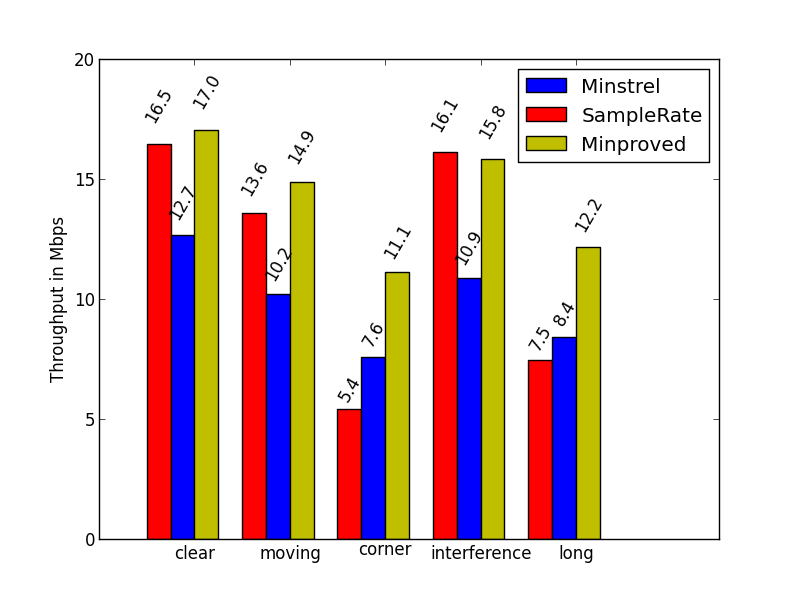
\includegraphics[width=3.5in]{mnVSspVSmp1.png}\vspace{-0em}
  \caption{Throughput of Minproved as compared to SampleRate and vanilla Minstrel.}
\label{figure:4}
\end{figure}


\subsection{Availability}
All of our code and collected trace data are available on GitHub:

\noindent
\small{\url{https://github.com/pavpanchekha/6.829-project/tree/3.8.6}}

This repository contains the modified ath9k driver used to collect the traces, the traces we collected, as well as the Python simulation framework. 

\section{Future Work}

Very little analysis has been done of the performance of bit rate selection algorithms on 802.11n networks. 802.11n introduces many new rates, as well as multiple-input/multiple output, or MIMO, capabilities. There is an 802.11n version of Minstrel, but there is no implmentation of SampleRate. 

We implemented SampleRate as outlined in the thesis, but the MadWifi implementation has a few key differences from the thesis. We suspect that the MadWifi use of an EWMA instead of a window has more accurate rate statistics, which will potentially lead to better throughput. We did not have the time to implement this alternative version, but it is worth further examination.

Hari Balikrishnan suggested that we use a broadcast approach when collecting our traces, instead of link layer acknowledgements. This would entail having multiple computers listening at the broadcast address, and compiling successes and failures from that information. This approach would free us from certain idiosyncracies of reading data from the driver, and lead to possibly more accurate traces. We were unable to implement this due to a lack of time and ability to acquire compatible hardware.

Finally, we are considering submitting our improvements to the Minstrel algorithm, namely the BEWMA, as a kernel patch. Currently is implemented in Python, so we would have to port the code into C.

\section{Conclusion}

Minstrel and SampleRate perform similarly. The results suggest that SampleRate tends to do slightly better, except in very lossy links such as the client being far awat from the AP or actively moving. Minproved, our improved version of Minstrel, solidly outperforms both Minstrel and SampleRate. 

It seems like the abandonment of SampleRate in the Linux kernel may have been a bit hasty, since it seems to perform similarly to Minstrel and it is a much simpler algorithm and thus less bug prone. We are not sure if there are adjustments to SampleRate that will bring it's performance near Minproved, though. 

\section{Acknowledgements}
We would like to thank Jonathan Perry and Hari Balikrishnan for their valuable guidance, as well as Derek Smithies for answering our questions about Minstrel. 


{\footnotesize \bibliographystyle{acm}
\bibliography{paper}}

\end{document}






